\documentclass[tikz,border=2pt]{standalone}
\usepackage{tikz}
\usetikzlibrary{arrows.meta,positioning}
\begin{document}
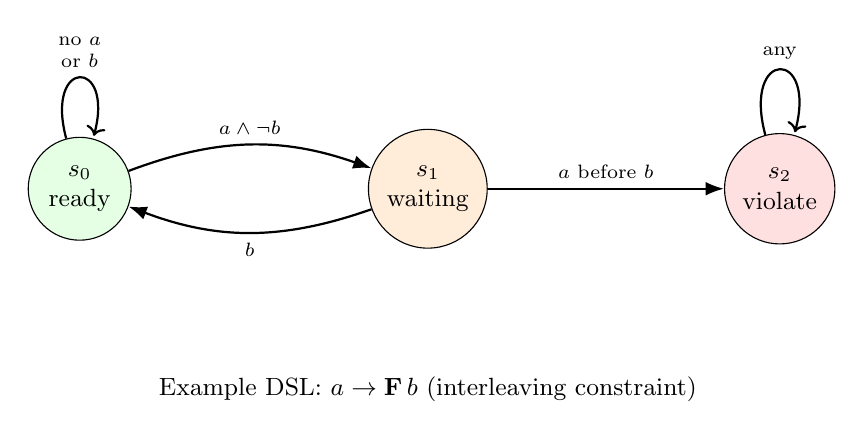
\begin{tikzpicture}[
  state/.style={draw, circle, minimum size=11mm, align=center, font=\small},
  ok/.style={state, fill=green!10},
  wait/.style={state, fill=orange!15},
  bad/.style={state, fill=red!12},
  arrow/.style={-{Latex}, thick},
]
  \node[ok] (s0) {$s_0$\\ready};
  \node[wait, right=30mm of s0] (s1) {$s_1$\\waiting};
  \node[bad, right=30mm of s1] (s2) {$s_2$\\violate};

  \draw[arrow] (s0) edge[loop above] node[font=\scriptsize, align=center]{no $a$\\or $b$} (s0);
  \draw[arrow] (s0) to[bend left=20] node[above, font=\scriptsize]{$a \wedge \neg b$} (s1);
  \draw[arrow] (s1) to[bend left=20] node[below, font=\scriptsize]{$b$} (s0);
  \draw[arrow] (s1) -- node[above, font=\scriptsize]{$a$ before $b$} (s2);
  \draw[arrow] (s2) edge[loop above] node[font=\scriptsize]{any} (s2);

  \node[below=15mm of s1, font=\small, align=center] {Example DSL: $a \to \mathbf{F}\, b$ (interleaving constraint)};
\end{tikzpicture}
\end{document}

